\section{MQTT}
Das \textbf{Message Queuing Telemetry Transport}, oder kurz \textbf{MQTT}, ist ein Protokoll, welches für die Kommunikation zwischen Maschinen bestimmt ist. Somit eignet sich dieses Protokoll auch im Wesentlichen für seinen Einsatz im Anwendungsbereich der Automatisierung und ganz besonders im Bereich des Internet der Dinge (\textbf{IoT} Internet of Things). Da aufgrund seines Aufbaus Geräte mit wenig Akkukapazität so gut wie keine eigene Rechenleistung erbringen müssen, um Nachrichten zu empfangen oder senden zu können, ist vor allem bei Akku-betriebenen Geräten ein Vorteil zu erkennen.\\
Erreicht wird dies durch den generellen Aufbau des Protokolls mittels Subscriber/ Publishern und einem zentralen Broker, wobei der Broker der verwaltende und Daten haltende Part ist und einem Server nahe kommt. Zudem gibt es die Subscriber, die Nachrichten empfangen können- ein Beispiel hierfür wären Aktoren. Die Publisher hingegen kommen zum Beispiel als Sensoren zum Einsatz, sie teilen der Netzwerkstruktur ihre Informationen mit. Die Einordnung als Subscriber oder als Publisher ist aber in keinem Fall exklusiv, sodass Geräte auch in einem hybriden Modus sowohl versenden als auch empfangen können, das wäre zum Beispiel bei einem Smart Home-Server der Fall.\\
 Ein ganz wesentlicher Vorteil des MQTT-Protokolls liegt in seiner Struktur als Publishing and Subcribe Verfahren. Dadurch, dass das Senden der Nachrichten nicht als Direktverbindung der Clients untereinander, sondern mit dem Umweg über den Broker geschieht, sind die Geräte in der Lage, Nachrichten sicher zu empfangen, auch wenn sie gerade nicht auf Nachrichten-Empfang stehen.\cite{b1}
 \begin{figure}[h]
 \caption{MQTT-Struktur \cite{b1}}
 \centering
 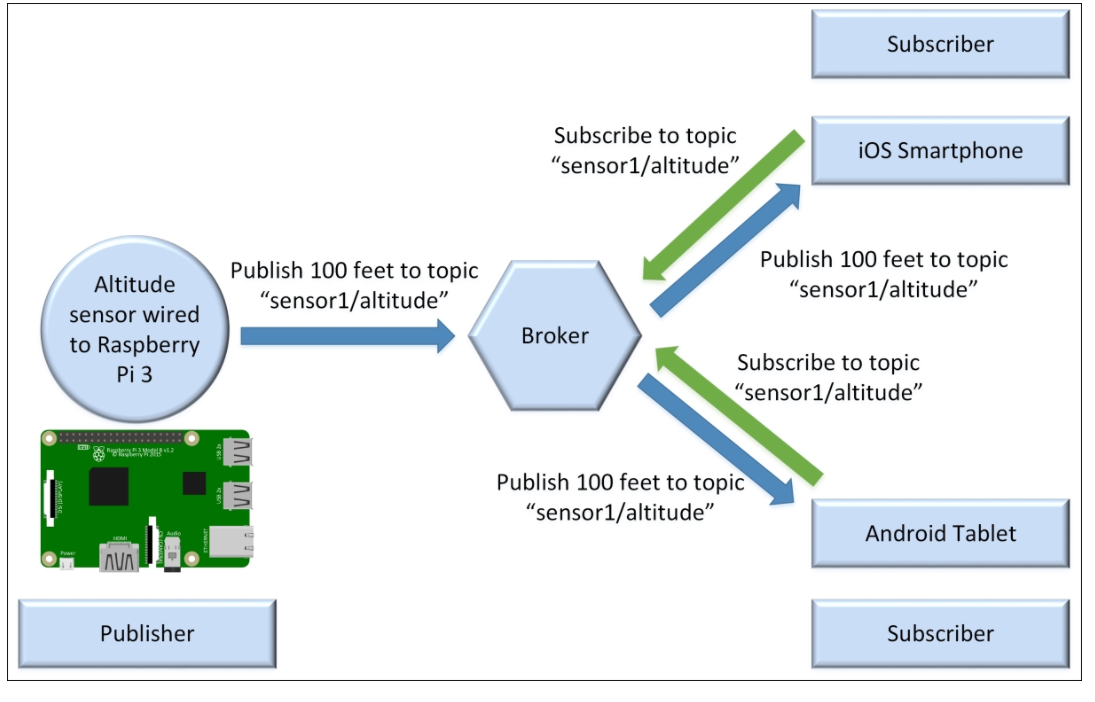
\includegraphics[scale=0.4]{mqtt_structure}
 \end{figure}
Jedoch bringt dieses Verfahren auch einen gravierenden Nachteil mit sich. Aufgrund dessen, dass Nachrichten nicht in einer eins-zu-eins-Übertragung miteinander geteilt werden, müssen Nachrichten auf eine andere Art und Weise zu ihrem Ziel gelangen. Fatal wäre hier zu glauben, auf eine Zuordnung der Nachrichten verzichten zu können. Da gerade in einem Smart Home viele ähnliche Geräte verbaut werden und somit auch viele ähnliche Werte versendet werden, wäre eine einfache Zuordnung nun nicht mehr ohne weiteres möglich.
Abhilfe schafft im MQTT-Protokoll ein Nachrichtenfilter mit einer Art Kanäle, die die Geräte "abonnieren" können, um nur relevante Daten zu erhalten\cite{b1}. Diese Kanäle haben Ähnlichkeit mit Adressen, geben Filter und Subfilter für die Nachrichtenverteilung an und werden nach dem Schema: \textsf{Erdgeschoss/Rolladensteuerung/Fenster1/Motor} erstellt, um ein Beispiel für die Ansteuerung des 1. Fensters im Erdgeschoss zu nennen. \\
Vorteile bietet MQTT des weiteren dank der Möglichkeit, das IP-Protokoll und somit TCP und TLS zu verwenden, was der Nachrichtenübertragung einen gewissen Schutz gegen das Verlieren von Nachrichten bietet, was gerade in kritischen Systembereichen einen Mehrwert hat. Und dank der Verschlüsselung mittels TLS bietet es einen Schutz gegen das zugreifen von unbefugten.